\chapter{Závěr}
Javascript je v současné době bezpochyby jedním z nejpoužívanějších jazyků vůbec. Tvoří důležitou část kódu v nepřeberném množství různých druhů moderních webových aplikací a stále nachází nové možnosti nejen na straně klienta, ale i na straně serveru. Vývojových prostředí a nástrojů pro ladění použitelných pro práci s Javascriptem je velké množství. Liší se od druhu zvolené implementace a většina je jich navržena pro použití Javascriptu na webu, ale začínají se objevovat také serverově nebo mobilně zaměřené nástroje. Velkým pokrokem byl také příchod konceptu jednostránkových webových aplikací (SPA), který přinesl kompletní implementaci aplikační logiky webové aplikace v prohlížeči pomocí Javascriptu.

V práci jsou představeny Single Page Aplikace, jejich princip a technické řešení spolu se souvisejícími technologiemi, které umožnily vývoj webových aplikací na této architektuře. Takové aplikace jsou potom naprosto závislé na podpoře Javascriptu, což přináší několik zásadních nevýhod. Největší z nich je špatná indexovatelnost SPA, protože roboti internetových vyhledávačů nepodporují Javascript. Tím pádem nevidí na stránce žádný text. Koncept isomorfních aplikací přenáší část zodpovědnosti z webového prohlížeče na webový server. Ten je zodpovědný především za vykreslování HTML, vyhledávací robot díky tomu získá již částečně zpracovanou stránku, která již obsahuje textový obsah. 

Vývoj isomorfních aplikací vyžaduje komplexnější architekturu a složitější vývojové prostředí než u klasických SPA. Jednostránkové webové aplikace často používají jeden monolitický framework, například Angular.js, zatímco ty isomorfní často využívají dokonce desítky menších knihoven, které vždy řeší jenom jednu oblast vývoje. Největší problém isomorfních aplikací je řešení přenosu prvotního aplikačního stavu vygenerovaného serverem do klientské části, běžící ve webovém prohlížeči. Tento princip se nazývá \textit{redyhratace} a často se řeší pomocí serializace vygenerováno stavu do javascriptové proměnné, kterou načte webový prohlížeč a následně celou aplikaci spustí. Toto řešení je použité také v ukázkové aplikaci, která je součástí této práce. Zjednodušeně tím dosáhneme toho, že načítání aplikace v prohlížeči začne přesně od bodu, kde skončilo serverové vykreslování. Druhým problémem je distribuce dat v aplikaci, není totiž možné používat automatický obousměrný data binding, tolik známý z frameworku Angular.js. To vyřešila společnost Facebook pomocí návrhového vzoru Flux, který řeší efektivní správu, aktualizaci dat a propagaci jejich změn. Isomorfní aplikace tedy představují evoluci jednostránkových aplikací, která řeší jejich hlavní problémy a zachovává vysoký stupeň interaktivity. Implementační rozdíly jsou však značné, především kvůli použití nového standardu Javascriptu zvaného ES6. Syntaktických změn je mnoho, jsou ale dobře popsány a jejich osvojení je pro schopného programátora otázka několika dní. Cílem práce bylo především popsat isomorfní přístup k programování webových aplikací v Javascriptu. Práce také demonstrovala využití těchto principů pomocí vytvořené ukázkové aplikace.

Existují však také názory, že isomorfní aplikace jsou přesně proti proudu doby. Je všeobecně známo, že každý programovací jazyk je vhodný pro trochu jiný typ aplikace. Z toho vyplývá, že by bylo vhodné využívat více programovacích jazyků pro různé oblasti vývoje. Například Jiří Knesl říká: \uv{Vázat se na jeden jazyk je hloupé. Správné řešení je použít tolik jazyků, kolik se vyplatí, ale zároveň nezbytné minimum} \cite{knesl}. Isomorfní přístup ale souvisí pouze s webovými aplikacemi, kde je dle mého názoru využití jednoho jazyka pro prohlížeč i server více než vhodné.

\section{Další směry výzkumu v oblasti}
Princip vývoje isomorfních webových aplikací je starý pouze několik let a stále se dynamicky vyvíjí. Mnoho přístupů není ještě plně standardizovaných. V této práci bylo cílem popsat pouze celkem ustálené a často používané principy. Tedy ty problémy, které byli ve světě isomorfních aplikací takřka vyřešeny. Další problémy se aktuálně řeší, komunita kolem isomorfních aplikací mimojiné přemýšlí například o nejvhodnějším způsobu definice CSS stylů. Vývojáři používající framework React doporučují deklarovat styly Javascriptem každému elementu zvlášť pomocí atributu \textit{style} (inline styly) \cite{react_css}, zatímco jiní vývojáři od tohoto přístupu odrazují \cite{inline_styles_hate}. 

Lze také očekávat větší zapojení Javascriptu do vývoje na mobilních zařízeních, především díky frameworkům jako React Native, které umožňují vyvíjet React aplikace pro mobilní telefony. Ty ale pro svůj běh nevyužívají mobilní internetový prohlížeč, jako je dnes u mobilních aplikací v Javascriptu běžné. Místo toho používají systémové UI komponenty dané mobilní platformy a ve výsledku se tak tváří jako nativní mobilní aplikace. React Native aplikace se programují v Javascriptu stejně jako běžné webové aplikace, ale místo HTML značek se zde využívají komponenty nativního uživatelského rozhraní. Programátor pak místo \textit{<div>} elementu použije element \textit{<View>}, který React Native přeloží do nativního kódu vzhledem k použité platformě (\textit{UIView} na iOS, nebo \textit{android.view} na Androidu). Všechny výhody React, především princip virtuálního DOM, jsou nyní dostupné i pro mobilní vývoj \cite{react_native}.

\pagebreak
Následující obrázek ilustruje fungování architektury React Native.
\vspace{0,3cm}
\begin{figure}[h]
\begin{centering}
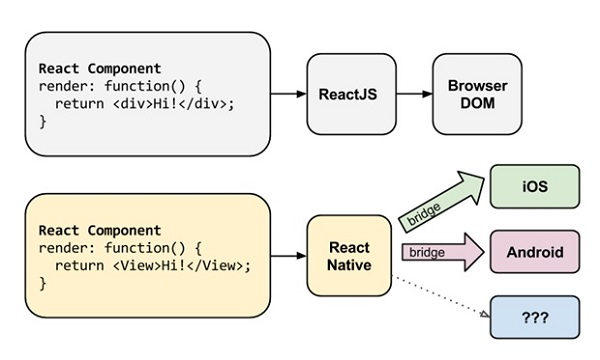
\includegraphics[scale=0.7]{obrazky/react_native}
\par\end{centering}
\caption{Diagram fungování frameworku React Native \cite{react_native_intro} \label{fig:react_native_intro}}
\end{figure}
\FloatBarrier